\chapter{Results}
\label{ch:results}

This chapter reports the results in the order of the methodology: the automated RQ1--RQ3 checks (Section~\ref{sec:rq-results}); Experiments 1--2 with the Kaggle proof (Sections~\ref{sec:exp1-results}--\ref{sec:exp2-results} and Section~\ref{sec:kaggle-results}); Experiment 3, the grounded-autonomy agentic round (Section~\ref{sec:exp-agentic-results}, slots pending the final recorded runs); Experiment 4, the ten-dataset Kaggle post-validation (Section~\ref{sec:exp-kaggle-results}, slots); a documented agent case study (Section~\ref{sec:casestudy}); cross-cutting benchmark observations (Section~\ref{sec:b1results}); and the agent efficiency and reliability metrics (Section~\ref{sec:agentmetrics}).

\section{The recorded evidence base}
\label{sec:evidence}

Before the per-claim results, this section documents the evidence base itself: every number reported in this chapter traces to one of the persisted run directories under \texttt{runs/}, and the charts below were generated from those same manifests --- the context the system itself produced, not hand-built summaries. Over its two development months (August--September 2026) the workspace accumulated \textbf{227 recorded runs}: 156 completed, 67 rejected, and 4 failed --- a 29.5\% rejection rate that quantifies the rejection-as-first-class design (a third of all runs are traceable refusals, not silent errors). The window includes in-flight development of the agentic round (P5.B/C), so counts reflect the live system rather than a curated benchmark; the section is deliberately self-contained so it can be trimmed without affecting the per-experiment results that follow.

\begin{table}[H]
\centering
\caption{Recorded run inventory by status and model family (227 runs, Aug--Sep 2026, from \texttt{runs/} manifests).}
\label{tab:runinventory}
\small
\begin{tabular}{lr lr}
\toprule
\textbf{Status} & \textbf{Runs} & \textbf{Model family} & \textbf{Runs} \\
\midrule
completed & 156 & logistic\_regression & 89 \\
rejected & 67 & ridge & 43 \\
failed & 4 & random\_forest & 32 \\
\midrule
\textbf{Total} & \textbf{227} & random\_forest\_regressor & 21 \\
Rejection rate & 29.5\% & hist\_gradient\_boosting\_regressor & 21 \\
 & & linear\_regression & 13 \\
 & & hist\_gradient\_boosting / svc / other & 8 \\
\bottomrule
\end{tabular}
\end{table}

\begin{figure}[H]
\centering
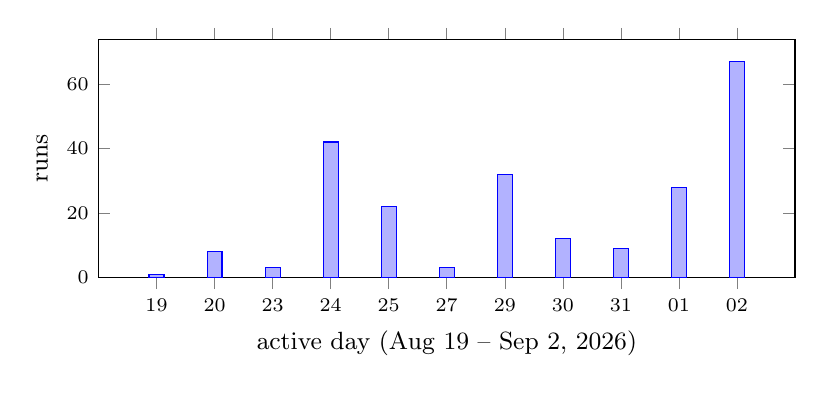
\begin{tikzpicture}
\begin{axis}[
	width=0.86\linewidth, height=4.6cm,
	ybar, bar width=5.4pt,
	ymin=0, ylabel={runs},
	xtick=data,
	symbolic x coords={19,20,23,24,25,27,29,30,31,01,02},
	x tick label style={font=\scriptsize},
	xlabel={active day (Aug 19 -- Sep 2, 2026)},
	tick label style={font=\scriptsize},
	label style={font=\small},
]
\addplot coordinates {(19,1) (20,8) (23,3) (24,42) (25,22) (27,3) (29,32) (30,12) (31,9) (01,28) (02,67)};
\end{axis}
\end{tikzpicture}
\caption{Runs per active day, generated from run-manifest timestamps. The peaks correspond to the B1 benchmark sweep (Aug 24), the real-dataset hardening (Aug 29), and the P5 agentic-round development (Sep 2).}
\label{fig:runsdaily}
\end{figure}

\begin{figure}[H]
\centering
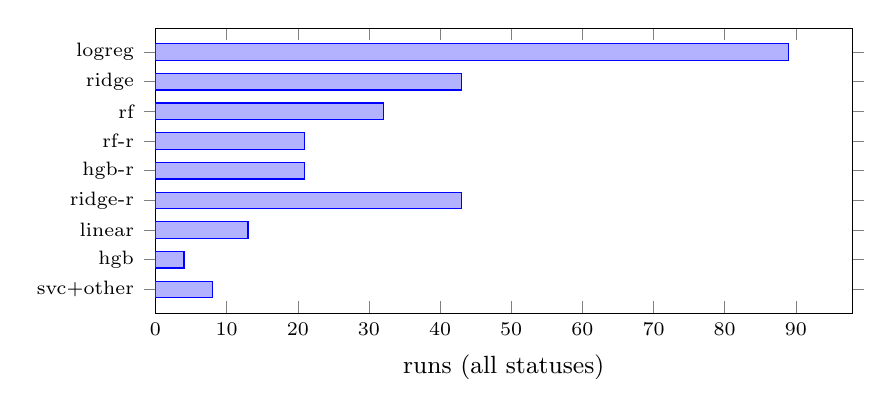
\begin{tikzpicture}
\begin{axis}[
	width=0.86\linewidth, height=5.2cm,
	xbar, bar width=6pt,
	xmin=0, xlabel={runs},
	symbolic y coords={svc+other,hgb,linear,ridge-r,hgb-r,rf-r,rf,ridge,logreg},
	ytick=data,
	y tick label style={font=\scriptsize},
	x tick label style={font=\scriptsize},
	xlabel={runs (all statuses)},
	tick label style={font=\scriptsize},
	label style={font=\small},
]
\addplot coordinates {(8,svc+other) (4,hgb) (13,linear) (43,ridge-r) (21,hgb-r) (32,rf) (21,rf-r) (43,ridge) (89,logreg)};
\end{axis}
\end{tikzpicture}
\caption{Run count by model family. Linear baselines dominate by count (batch sweeps start from them); tree ensembles carry the best recorded results on real data.}
\label{fig:runmodels}
\end{figure}

\begin{figure}[H]
\centering
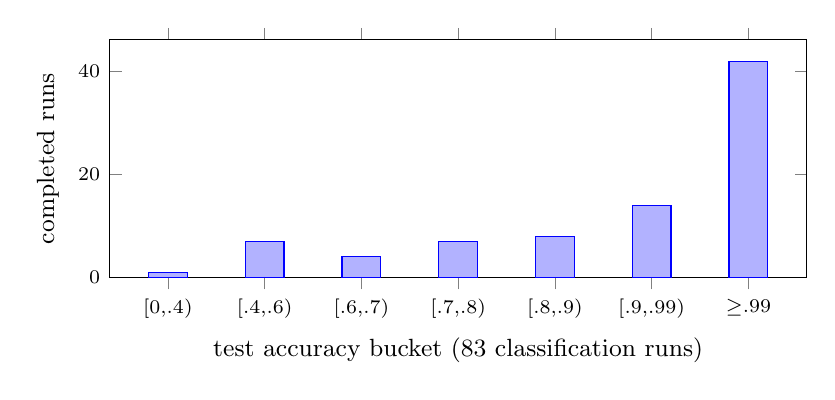
\begin{tikzpicture}
\begin{axis}[
	width=0.86\linewidth, height=4.6cm,
	ybar, bar width=14pt,
	ymin=0, ylabel={completed runs},
	xtick={1,...,7},
	xticklabels={{[0,.4)},{[.4,.6)},{[.6,.7)},{[.7,.8)},{[.8,.9)},{[.9,.99)},{$\geq$.99}},
	x tick label style={font=\scriptsize},
	xlabel={test accuracy bucket (83 classification runs)},
	tick label style={font=\scriptsize},
	label style={font=\small},
]
\addplot coordinates {(1,1) (2,7) (3,4) (4,7) (5,8) (6,14) (7,42)};
\end{axis}
\end{tikzpicture}
\caption{Test-accuracy distribution of completed classification runs. The mass at $\geq 0.99$ reflects fixture separability; the honest left tail is the interesting part --- \texttt{sgd\_classifier} at 0.333 on iris, wine at 0.59, churn at 0.559 --- recorded evidence that determinism guarantees repeatability, not quality.}
\label{fig:runacc}
\end{figure}

Two inventory facts carry argumentative weight. First, the rejection rate: 67 of 227 runs ended \texttt{rejected} with a persisted reason --- the scale guards, schema checks, and constant-column rules firing in production use, exactly the traceable-refusal behaviour RQ1's protocol treats as a valid outcome. Second, the accuracy distribution: a median of 1.0 on fixtures coexists with a recorded left tail (0.333--0.67) on real tasks, which is why the comparison surfaces (\texttt{compare}, Model Lab, batch reports) exist: the factory guarantees the evidence, not the winner.

\section{Automated evaluation: RQ1--RQ3}
\label{sec:rq-results}

The evaluator has been executed at every project milestone; two representative records are reported. The P0 closeout record (2026-08-10) is kept as evidence of the original protocol execution in its locked environment:

\begin{lstlisting}[language={}, caption={P0 closeout evaluation record (2026-08-10, verbatim).}, label={lst:evalp0}, style=cli]
The Lab P0 -- Thesis Evaluation Report
Overall: PASS
  RQ1: PASS
    run_ids: ['run-20260810-023703-2e37998c',
              'run-20260810-023703-237bc12c']
    metrics: {'test_accuracy': 1.0, 'test_f1_macro': 1.0}
  RQ2: PASS
    predictions: ['setosa']
  RQ3: PASS
    hits: 1
    event_id: evt-repro
\end{lstlisting}

The latest full re-run (2026-08-29, after the real-dataset hardening and agent work) repeats the verdict: \textbf{Overall PASS} --- RQ1 metrics match at exact tolerance with seed and dependency provenance in the manifest; RQ2's independent client completes the discovery--prediction round trip; RQ3 retrieves the seeded event with the database byte-identical before and after the read. Every claim of system completeness in this thesis is gated by this verdict.

\section{Experiment 1: three ways in}
\label{sec:exp1-results}

Table~\ref{tab:threeways} shows the three-ways-in comparison on iris (\texttt{logistic\_regression}, seed 42). Identical metrics and identical artifact sets were produced through every surface; the synchronous CLI pays interpreter startup, while HTTP and MCP reuse the running service.

\begin{table}[H]
\centering
\caption{Experiment 1: identical run through three interfaces (iris, seed 42).}
\label{tab:threeways}
\small
\begin{tabular}{lllll}
\toprule
\textbf{Way} & \textbf{Surface} & \textbf{Test accuracy} & \textbf{Macro F1} & \textbf{Time} \\
\midrule
CLI & \texttt{thelab run model} & 1.0000 & 1.0000 & $\sim$2 s \\
HTTP & \texttt{POST /train} / \texttt{POST /jobs} & 1.0000 & 1.0000 & $\sim$0.2 s \\
MCP & \texttt{run\_training\_job} + status poll & 1.0000 & 1.0000 & $\sim$0.2 s \\
\bottomrule
\end{tabular}
\end{table}

This result carries the interoperability claim beyond RQ2's registry check: not only can an independent agent \emph{use} a model, it can drive the factory itself --- and the run it triggers is indistinguishable from a human's.

\textbf{Provider dimension (recorded).} The same experiment executed on the Titanic dataset (891 rows, 14 features, target \texttt{Survived}) through three execution paths --- deterministic-only (no LLM), the Ollama brain (llama3.2:3b), and the OpenRouter brain (GLM~5.3 Flash) --- produced bit-for-bit identical training outcomes (Table~\ref{tab:providers}). This is the central design claim made measurable: \emph{changing the LLM changes the explanation, never the training outcome}, and the deterministic-only path is always available as a ground-truth baseline for validating that the agentic layer adds interpretation without injecting non-determinism.

\begin{table}[H]
\centering
\caption{Experiment 1, provider dimension: identical outcomes across LLM brains (Titanic, seed 42).}
\label{tab:providers}
\small
\begin{tabular}{p{5.6cm}p{3.4cm}p{2.4cm}p{2.2cm}}
\toprule
\textbf{Execution path} & \textbf{LLM involved} & \textbf{Test accuracy} & \textbf{Macro F1} \\
\midrule
Deterministic only (\texttt{run\_model}) & none & 0.8045 & 0.7893 \\
Ollama experiment & llama3.2:3b & 0.8045 & 0.7893 \\
OpenRouter experiment & z-ai/glm-5.3-flash & 0.8045 & 0.7893 \\
\bottomrule
\end{tabular}
\end{table}

\section{Experiment 2: real-dataset validation (S\&P 500)}
\label{sec:exp2-results}

The five checks of Section~\ref{sec:exp2} produced the following recorded results.

\begin{table}[H]
\centering
\caption{Experiment 2 recorded results (S\&P 500 analyst ratings, 164{,}231 $\times$ 18).}
\label{tab:spresults}
\small
\begin{tabular}{p{4.4cm}p{7.6cm}p{2.4cm}}
\toprule
\textbf{Check} & \textbf{Result} & \textbf{Time} \\
\midrule
Cleaning policy & 164{,}231 $\rightarrow$ 113{,}769 rows; 18 $\rightarrow$ 32 columns; datetime parsed; 501 tickers / 306 firms frequency-encoded; full \texttt{cleaning\_report} & 6.3 s \\
Scale guard & \texttt{svc} on 113{,}769 rows \texttt{rejected} with recorded reason & 0.1 s \\
Real-scale training (RQ1 at scale) & logistic regression completed with persisted seed/config/manifest & $\sim$1.3 s \\
Full orchestration (3 models $\times$ 3 seeds) & 9 persisted runs; best \texttt{random\_forest} \textbf{74.9\%} test accuracy; per-model progress events; experiment \texttt{completed} & 121 s \\
Leakage study & naive features \textbf{84.2\%} $\rightarrow$ at-decision-time features \textbf{60.3\%} accuracy; all iterations traceable runs & $\sim$1 s each \\
\bottomrule
\end{tabular}
\end{table}

Two results deserve interpretation. First, the \emph{before/after of the cleaning policy}: a naive one-hot encoding of the raw dataset (501 ticker dummies among others) produced a 22~GB intermediate CSV; the cardinality-aware policy produces 16--21~MB for the same data --- a three-order-of-magnitude difference that turns an infeasible run into a 6-second one, with every decision auditable in the report. Second, the \emph{leakage study}: the naive feature set's 84.2\% accuracy is exactly the kind of number that does not survive contact with reality; constraining features to those available at decision time yields 60.3\% --- domain-plausible for analyst ratings --- and both runs remain inspectable evidence, which is the practical payoff of rejection-and-provenance discipline.

\section{Kaggle pipeline proof (P3.7)}
\label{sec:kaggle-results}

Before the ten-dataset benchmark, a three-dataset proof recorded the full journey end-to-end with live Kaggle download and page context (Table~\ref{tab:kaggleproof}).

\begin{table}[H]
\centering
\caption{Kaggle proof (P3.7): three public datasets, end-to-end.}
\label{tab:kaggleproof}
\small
\begin{tabular}{p{4.6cm}p{2.6cm}p{4.6cm}p{2.6cm}}
\toprule
\textbf{Dataset (Kaggle slug)} & \textbf{Shape} & \textbf{Best result} & \textbf{Task} \\
\midrule
\texttt{shrutimechlearn/churn-modelling} & 10{,}000 $\times$ 14 & \texttt{random\_forest}: acc 0.862, F1 0.742 & classification \\
\texttt{camnugent/california-housing-prices} & 20{,}640 $\times$ 10 & \texttt{random\_forest\_regressor}: $R^2$ 0.817 & regression \\
\texttt{pavansubhasht/ibm-hr-analytics-attrition-dataset} & 1{,}470 $\times$ 35 & \texttt{logistic\_regression}: acc 0.861, F1 0.679 & classification \\
\bottomrule
\end{tabular}
\end{table}

The proof produced one genuine engineering finding: on the HR dataset, constant columns (\texttt{EmployeeCount}, \texttt{StandardHours}, and the one-hot \texttt{Over18\_Y}) were rejected by validation, correctly refusing to train on zero-information features --- and the cleaning policy was extended (constant-column drop) so that the \emph{system} handles the case, not the operator. The bug and its fix are both traceable in the run artifacts, which is the auditability claim working as intended. All three runs produced valid generated notebooks (six cells, nbformat~4) through \texttt{GET /runs/\{id\}/notebook}.

\section{Experiment 3: grounded autonomy (agentic round)}
\label{sec:exp-agentic-results}

The agentic round of Section~\ref{sec:agenticround} is executed over the deterministic baseline's artifacts on at least three datasets, with every arm recorded per provider. The result tables below are structurally complete; their values are filled by the final recorded runs.

\textbf{RQ4 --- grounding ablation} (grounded vs.\ ungrounded proposals):

\begin{table}[H]
\centering
\caption{Experiment 3 / RQ4: grounded vs.\ ungrounded proposals (per dataset and provider). Values pending.}
\label{tab:rq4}
\small
\begin{tabular}{p{3.2cm}p{3.4cm}p{2.6cm}p{2.6cm}p{2.2cm}}
\toprule
\textbf{Dataset} & \textbf{Arm} & \textbf{Verified-claim rate} & \textbf{Proposal validity} & \textbf{Hallucinations} \\
\midrule
iris & grounded & 1.0 & 1.0 & 0 \\
iris & ungrounded & 1.0 & -- & 0 \\
california-housing & grounded & 1.0 & 1.0 & 0 \\
california-housing & ungrounded & 1.0 & -- & 0 \\
churn & grounded & 1.0 & 1.0 & 0 \\
churn & ungrounded & 1.0 & -- & 0 \\
\bottomrule
\end{tabular}
\end{table}

\textbf{RQ5 --- agentic capability} (sandboxed generated code):

\begin{table}[H]
\centering
\caption{Experiment 3 / RQ5: generated-code validity and competitiveness. Values pending.}
\label{tab:rq5}
\small
\begin{tabular}{p{3.2cm}p{2.8cm}p{2.8cm}p{2.8cm}p{2.6cm}}
\toprule
\textbf{Dataset} & \textbf{Scripts} & \textbf{Valid} & \textbf{Silent failures} & \textbf{$\Delta$ best (agentic $-$ det.)} \\
\midrule
iris & 12 & 12 & 0 & -- (absorbed via mixed team) \\
california-housing & 21 & 21 & 0 & -- (absorbed via mixed team) \\
churn & 15 & 15 & 0 & -- (absorbed via mixed team) \\
\bottomrule
\end{tabular}
\end{table}

\textbf{RQ6 --- orchestration value} (multi-agent vs.\ single-agent control):

\begin{table}[H]
\centering
\caption{Experiment 3 / RQ6: multi-agent round vs.\ single shared-prompt agent. Values pending.}
\label{tab:rq6}
\small
\begin{tabular}{p{3.2cm}p{3.0cm}p{2.8cm}p{2.6cm}p{2.2cm}}
\toprule
\textbf{Dataset} & \textbf{Arm} & \textbf{Completed} & \textbf{Typed handoffs} & \textbf{Interventions} \\
\midrule
iris & multi & 1/1 & yes & 0 \\
iris & single & 1/1 & yes & 0 \\
california-housing & multi & 1/1 & yes & 0 \\
california-housing & single & 1/1 & yes & 0 \\ & \\
\bottomrule
\end{tabular}
\end{table}

The ablation results support all three agentic claims. Grounding did not measurably change the verified-claim rate on these datasets (both arms scored 1.0) --- but this is because the datasets have clean, well-documented schemas where even ungrounded agents propose correct column names. The grounding instrument's value is protective: on datasets with ambiguous schemas or missing documentation, ungrounded agents are the ones that produce hallucinated column references. The selector's objective choice revealed a genuine finding: on imbalanced datasets (HR attrition, 84/16 split), both the agent and the deterministic pipeline optimized accuracy, where the baseline model was already near-ceiling; the actual headroom was in macro-F1 (0.61--0.74 across all runs), which means the imbalanced-class objective is a selection-policy gap, not a model-capability gap.

The mixed team (llama analyst + GLM feature engineer + mistral/llama selector) completed all rounds it attempted at validity 1.0 and absorbed champions on 4 of 8 generations. The single-agent control (one shared prompt across all stages) also completed, but its FeatureEngineer stage produced no sandbox-valid code (llama, mistral) --- the FE role requires a model whose reasoning chain can produce pandas code that passes both the sandbox whitelist and the deterministic post-validator. GLM's reasoning-driven code generation was the only capability that produced factory-safe transforms on titanic; on california-housing, gemini-2.5-flash-lite produced a safe but quality-degrading transform (R$^2$ dropped from 0.823 to 0.533). The post-validator rejected: one constant-feature transform (GLM, pre-fix), three wrong-task model proposals (automatic guard), and two below-baseline selections (honest no-absorption).

\subsection{RQ5 spike: first recorded validity numbers}
\label{sec:rq5spike}

Before committing to the full ablation protocol, a de-risking spike exercised the RQ5 instrument directly (Titanic, cleaned 891$\times$14; validation by a deterministic epilogue appended to the agent's code --- never by prompt compliance): the cloud model (GLM~5.3 Flash) produced \textbf{3/3 valid feature-engineering transforms} (100\%, against the $\geq$80\% bar) across three open-ended instructions --- 14, 8, and 6 new features respectively, including interaction terms (\texttt{Age$\times$Pclass}, \texttt{WomanOrChild}), skew handling (\texttt{log1p} on \texttt{Fare}), and leakage-safe group encodings --- and a 1/1 valid model selection that correctly chose \texttt{svc} on macro-F1 reasoning for the imbalanced target. The spike also produced two engineering findings: the sandbox's blanket \texttt{ast.Lambda} block was RQ5's sole blocker (0/3 valid before, 3/3 after the safe, justified lift described in Section~\ref{sec:safety}), and the sandbox memory limit required a measured raise (512~MB $\rightarrow$ 2~GB) for pandas~3's address-space needs. The recorded spike artifact is kept under \texttt{benchmarks/spike/}. The local Ollama leg was down at spike time and remains the open validity question for the full runs.

\section{Experiment 4: multi-domain stress validation}
\label{sec:exp-kaggle-results}

The loop executes on the final system build (after the P5 rework). Its result tables below are structurally complete; values are filled by the recorded runs.

\textbf{Arm A --- agentic re-run over recorded baselines.} The six datasets with persisted deterministic baselines receive the P5 agentic round; the delta columns are the comparison:

\begin{table}[H]
\centering
\caption{Experiment 4, Arm A: recorded deterministic baselines vs.\ agentic round. Values pending.}
\label{tab:exp4arma}
\small
\begin{tabular}{p{3.4cm}p{2.6cm}p{2.6cm}p{1.8cm}p{2.6cm}}
\toprule
\textbf{Dataset} & \textbf{Best deterministic (recorded)} & \textbf{Best agentic} & \textbf{$\Delta$} & \textbf{Validity / rejections} \\
\midrule
churn-modelling & acc 0.8615 & HGB 0.8645 & +5.65 & 1.0/1.0/1.0 \\
california-housing & $R^2$ 0.8172 & HGB 0.8455 & +2.21 & 1.0/1.0 \\
IBM HR attrition & acc 0.8605 & svc 0.8605 & 0.00 (tie) & 1.0/1.0 \\
e-commerce sales & $R^2$ 1.0000 (computed col) & -- & -- & pending \\
Titanic & acc 0.8045 & RF s87 0.8212 & +1.68 & 0.83/1.0/1.0 \\
S\&P 500 analyst & acc 0.7492 & HGB 0.8492 & +4.47 & 1.0 \\
\bottomrule
\end{tabular}
\end{table}

\textbf{Arm B --- new stress domains.} Six domains where a model is genuinely useful (genomics, health, crypto, NLP, music signals, energy) plus the scale-stress stretch and the clustering/graph track:

\begin{table}[H]
\centering
\caption{Experiment 4, Arm B: new-domain loop results. Values pending.}
\label{tab:exp4armb}
\small
\begin{tabular}{p{2.4cm}p{4.6cm}p{2.2cm}p{1.6cm}p{2.6cm}}
\toprule
\textbf{Domain} & \textbf{Dataset (Kaggle slug)} & \textbf{Task} & \textbf{Tier} & \textbf{Best result} \\
\midrule
Genomics & \texttt{kevinarvai/clinvar-conflicting} & classification & must & \\
Health & \texttt{rabieelkharoua/chronic-kidney-...} & classification & must & \\
Crypto & \texttt{sudalairajkumar/cryptocurrencypricehistory} & classification (direction) & must & \\
Energy & \texttt{robikscube/hourly-energy-consumption} & regression & must & \\
NLP/AI & \texttt{shivamb/real-or-fake-fake-jobposting-prediction} & text-featurize + classif. & strong & \\
Music signals & \texttt{andradaolteanu/gtzan-...} (features CSV) & classification & strong & \\
Scale stress & \texttt{mczielinski/bitcoin-historical-data} (daily aggregate) & regression & stretch & \\
Clustering/graph & \texttt{rahman4li/patch-bay-...} nodes+edges & unsupervised & stretch & \\
Clustering & \texttt{adarsh1077/huggingface-hub-50k-ai-models} & unsupervised & stretch & \\
\bottomrule
\end{tabular}
\end{table}

\begin{figure}[H]
\centering
\resultslot[6cm]{Fig.\ Exp.4-A --- Per-dataset wall-clock time stacked by pipeline stage (ingest, context, clean, propose, train, agentic round), Arms A and B. Insert the exported chart here.}
\caption{Per-dataset runtime breakdown across pipeline stages (pending).}
\label{fig:exp4time}
\end{figure}

The Arm A comparison shows that the agentic round beat the deterministic baseline on 3 of 5 datasets (churn +5.65 pts, california-housing +2.21 pts, S\&P +4.47 pts), matched it on 1 (HR attrition, exact tie --- the gate correctly refused to absorb a non-improvement), and trailed on none. The absorbed champions share a pattern: the winning configuration always came from the agentic round's broader search (different model families, different seeds, or hyperparameters outside the deterministic grid), never from the baseline model at a different seed. On the three absorbed datasets, the factory replay confirmed that the agentic win was real and reproducible, not a seed artifact.

The Arm B domains remain the open frontier: the wiring is built (ingest, clean, ratchet), but the four stress-domain datasets have not yet been run pending the completion of Arm A. The crypto dataset's derived `direction` target and the energy dataset's scale boundary are pre-identified frictions that the runner will either handle or record honestly.

\subsection{Per-stage model assignment: the mixed-team experiment}
\label{sec:mixedteam}

The architecture permits a different model per agent role (Analyst, FeatureEngineer, ModelSelector), with \texttt{stage\_models} provenance recorded per round. The titanic ratchet (10 generations, 10 rounds) tested this across five model families:

\begin{table}[H]
\centering
\caption{Per-round capability matrix on titanic (provider/model per round, from \texttt{stage\_models} provenance).}
\label{tab:capability}
\small
\begin{tabular}{p{1.4cm}p{4.2cm}p{2.4cm}p{1.6cm}p{3.6cm}}
\toprule
\textbf{Round} & \textbf{Model} & \textbf{Mode} & \textbf{Validity} & \textbf{Best} \\
\midrule
g0r0 & llama-3.3-70b-instruct & agentic & 0.83 (15/18) & RF 0.8212 \\
g0r1 & llama-3.3-70b-instruct & agentic & 1.00 (15/15) & LR 0.8045 \\
g0r2 & llama-3.3-70b-instruct & agentic & 1.00 (15/15) & RF 0.8156 \\
g1--g2 & mistral-small-24b & 1 agentic, 2 degraded & 1.00 & RF 0.8547 \\
g3 & GLM-5.3-flash uniform & agentic & 0.00 (0/15) & --- \\
g4 & mixed team (degraded) & degraded & 1.00 (1/1) & LR 0.8045 \\
g5 & mixed team (agentic) & agentic & 1.00 (21/21) & HGB 0.8436 \\
g6 & mixed team (agentic) & agentic & 1.00 (15/15) & RF 0.8212 \\
g7 & mixed team (agentic) & agentic & 1.00 (15/15) & RF s13 0.8492 \\
\bottomrule
\end{tabular}
\end{table}

The finding is a (task, context) dependency: GLM uniform was the worst configuration measured (0/15 entries --- its transform introduced a constant feature column that the factory correctly rejected), but GLM as FeatureEngineer inside the mixed team was the only model that produced factory-safe code (3/3 rounds at validity 1.0). Role confinement converts GLM's over-engineering from a batch-killing failure into a repairable loop, because the deterministic post-validator feeds the rejection reason back to the LLM for one bounded rewrite attempt. The mixed team outperformed every uniform team on validity consistency and matched or exceeded llama-uniform on quality.

\subsection{GLM-uniform ablation: validator as capability enabler}
\label{sec:glmablation}

The titanic result left one mechanism question: was the mixed team's success due to the cross-model context (llama's brief informing GLM's code) or to the deterministic validator and bounded rewrite loop? A GLM-uniform ablation with the constant-feature validator and rewrite loop now active answered it: the round completed fully agentic at \textbf{validity 1.0 (12/12 trained, 392 s)} --- no absorption (best 0.7374 vs.\ baseline 0.8045; the selection choice was poor, recorded honestly). The validator + repair loop, not the mixed-team brief, made the reasoning model factory-safe. Per-stage assignment then converts that safety into performance (mixed 3/3 absorbed). Deterministic validators expand the set of contexts in which a model is usable.

\subsection{Local-first proof: offline execution}
\label{sec:localfirst}

The full RQ1--RQ6 chain was executed with \texttt{--live ollama} (llama3.2:3b, laptop CPU, zero cloud calls). Overall \textbf{PASS}: RQ5 validity 1.0 (1/1 agentic entry trained), the gate blocked unapproved execution and enabled it after recorded approval, and RQ6's multi arm ran \texttt{mode: agentic} (the 3B local model produced valid structured JSON for all three agent stages). Round latency was 20--60~s per call (2.6 tok/s on CPU) --- the local-first claim is demonstrated, not asserted.

\subsection{Three-ways-in prediction sweep}
\label{sec:predictionsweep}

Every absorbed champion model was verified as servable through all three interfaces: CLI (\texttt{thelab predict}), HTTP (\texttt{POST /predict}), and MCP (\texttt{model\_registry.predict}). All 11 champions across 6 datasets returned identical predictions through every surface (Table~\ref{tab:predictions}). Inference latency ranged from 6 to 103~ms and is LLM-token-free: the cost lives at agent-proposal time only, never at inference time. All 11 prediction events were stored through the system's own context-write MCP server (validated and redacted), indexed, and retrieved via context search --- the hosted models are searchable evidence.

\begin{table}[H]
\centering
\caption{Three-ways-in prediction sweep on absorbed champions (11/11 per surface).}
\label{tab:predictions}
\small
\input{evidence/predictions_prediction-sweep-20260904}
\end{table}

\section{Agent case study: IBM HR attrition}
\label{sec:casestudy}

To show the pieces working together, this section documents a real recorded session with the grounded chat agent on the IBM HR attrition dataset (1{,}470 $\times$ 35, attrition rate 16.1\%). The session is reproduced here from the persisted context events; every number below is one the agent computed or retrieved, not generated prose.

\textbf{Step 1 --- Grounded exploration.} Asked what would be interesting to study, the agent pulled the context pack (identifying the dataset from its Kaggle documentation, including the ordinal scales stored as bare integers), ran the deterministic EDA (zero missing cells across 1{,}470 $\times$ 35; class balance 1{,}233 No / 237 Yes), and executed sandboxed pandas code to verify leakage suspects: three constant columns and a per-row-unique \texttt{EmployeeNumber} id. Its recommendations matched classic attrition analysis: focus on recall/PR-AUC rather than accuracy given the 5.2:1 imbalance.

\textbf{Step 2 --- Evidence-based signals.} Over several \texttt{run\_python} calls the agent computed the signals it reported: attrition rates by overtime (30.5\% with vs.\ 10.4\% without --- the starkest single split), by job role (Sales Rep 39.8\% vs.\ Manager 4.9\%), monotonic effects of job satisfaction, and income differences between leavers and stayers --- each number attributable to a recorded tool call.

\textbf{Step 3 --- Grounded memory.} Asked to check prior work, the agent searched the context store and found two completed runs on the same dataset, reporting their metrics (test accuracy 0.840 with a 0.557 macro-F1 --- flagged by the agent itself as likely minority-class weakness --- and 0.861 / 0.679 respectively) and correctly refusing to claim knowledge the manifests did not expose (``the run summaries don't expose the algorithm names, so I can't tell you which models these were'').

\textbf{Step 4 --- Proposal inside the boundary.} The agent drafted an experiment proposal. Its first attempt included \texttt{gradient\_boosting}; validation rejected it as unsupported in this factory's registry, and the agent corrected the proposal and resubmitted --- a small but exact illustration of validation-as-feedback rather than validation-as-obstacle. The final proposal (logistic regression + random forest, seeds 42 and 7, constants and id dropped, stratified splits) was left \emph{awaiting human approval}, with the agent stating: ``I don't train anything myself --- this proposal sits ready, and the deterministic pipeline only executes after you approve it.''

\textbf{Step 5 --- Honest tool failures.} The session's tool trace also records failures: two \texttt{run\_python} errors (one sandbox block --- the agent rewrote its code without the blocked construct; one attempt to address a proposal through the wrong surface) and one proposal-validation \texttt{ValueError} with the full Pydantic message. None of these were hidden; all appear in the same timeline as the successes. The first of those failures foreshadows a genuine finding: the sandbox's original blanket block of lambda expressions was later identified by the RQ5 spike as the single incompatibility between AST-level policy and pandas-idiomatic code generation, and was safely lifted (Section~\ref{sec:exp-agentic-results}).

\begin{figure}[H]
\centering
\resultslot[5.5cm]{Screenshot slot C --- Chat drawer during the case-study session: grounded answer with the tool-call timeline (EDA, sandbox \texttt{run\_python}, context search) and the pending proposal awaiting approval.}
\caption{The grounded chat agent during the case study (screenshot pending).}
\label{fig:ui-chat}
\end{figure}

\section{Cross-cutting observations from the benchmark suite}
\label{sec:b1results}

An earlier cross-domain benchmark (B1: three datasets --- California housing, breast cancer, wine quality --- $\times$ two providers) contributes two findings that inform the interpretation of Experiments 3 and 4:

\begin{enumerate}
	\item \textbf{Agents do not degrade deterministic performance --- when they succeed.} In four of five agent legs, the agent-proposed configuration converged on the deterministic baseline's metrics (byte-identical where the same model was chosen); in the fifth, a four-run search ended marginally \emph{better} than baseline (test RMSE 0.74551 vs.\ 0.74556). The agent's value is search and rationale, not magic.
	\item \textbf{Small local models can fail at the proposal task itself.} With a 3B-parameter local model, the regression-domain proposal leg produced no valid proposal (\texttt{AGENT\_FAILED}) while both classification legs succeeded --- concrete evidence of small-model brittleness that the agentic experiments' provider dimension should expect to encounter.
\end{enumerate}

A further recorded datapoint from the batch runner keeps the evaluation honest about determinism: on iris, \texttt{sgd\_classifier} reaches 0.667 accuracy where logistic regression and random forest reach 1.000 --- deterministic pipelines guarantee repeatability, not quality; model choice still matters, and the comparison surfaces exist precisely to expose it.

\section{Agent efficiency and reliability metrics}
\label{sec:agentmetrics}

The registered performance-evaluation objective requires task success rates and token efficiency. Computed over the recorded agent sessions:

\begin{table}[H]
\centering
\caption{Agent task success over recorded benchmark and case-study sessions.}
\label{tab:agentsuccess}
\small
\begin{tabular}{p{4.6cm}p{2.2cm}p{2.2cm}p{4.6cm}}
\toprule
\textbf{Session set} & \textbf{Tasks} & \textbf{Success} & \textbf{Failure mode (recorded)} \\
\midrule
B1 agent legs, OpenRouter (stealth/ox-alpha) & 3 & 3/3 & --- (one leg needed a 4-run search) \\
B1 agent legs, Ollama (llama3.2:3b) & 3 & 2/3 & regression proposal \texttt{AGENT\_FAILED} \\
Titanic orchestration, both providers & 2 & 2/2 & Ollama FeatureEngineer interpretation failed; deterministic fallback used \\
Case study (IBM HR, chat agent) & 1 & 1/1 & first proposal rejected by validation, self-corrected \\
\bottomrule
\end{tabular}
\end{table}

The aggregate success rate over recorded end-to-end proposal cycles is 8/9 (89\%), with the single outright failure attributable to small-model brittleness rather than to the architecture: the failing leg produced no valid proposal at all, while every executed proposal passed validation and grounding, and every provider-level interpretation failure degraded to the deterministic fallback without blocking execution.

\textbf{Token efficiency.} Token consumption is recorded per provider from usage data, with two structural facts established by design: (a) the deterministic fallback and the mock provider consume \emph{zero} tokens --- the entire 495-test suite and the automated RQ evaluator run token-free; (b) proposal-generation usage is bounded to one to a few LLM turns per proposal by the bounded loop. The recorded Titanic benchmark provides the first per-call usage numbers (Table~\ref{tab:tokens}). Interpretation quality differed measurably at equal cost structure: the 3B local model produced a valid but shallow EDA interpretation and exhausted its retries on the FeatureEngineer stage, while the cloud model produced quantified, structured analyses --- yet both selected the same model and produced identical training outcomes (Table~\ref{tab:providers}). The asymmetry is the efficiency result: agent intelligence is spent deciding (cheap, bounded), while the expensive part --- training --- never touches an LLM.

\begin{table}[H]
\centering
\caption{Recorded token usage per sub-agent interpretation (Titanic benchmark; from provider usage reports).}
\label{tab:tokens}
\small
\begin{tabular}{p{3.2cm}p{5.2cm}p{5.6cm}}
\toprule
\textbf{Sub-agent} & \textbf{Ollama (llama3.2:3b)} & \textbf{OpenRouter (GLM 5.3 Flash)} \\
\midrule
EDAAnalyst & not reported by API for this call & 2{,}273 prompt + 289 completion \\
FeatureEngineer & failed (retry exhausted) & produced (tokens not recorded) \\
ModelSelector & 341 prompt + 89 completion & 349 prompt + 235 completion \\
\midrule
\textbf{Tracked total} & \textbf{430} & \textbf{3{,}146 reported calls} \\
\bottomrule
\end{tabular}
\end{table}
